%
\documentclass[12pt,letter]{article}

\usepackage[utf8]{inputenc}
\usepackage[usenames,dvipsnames]{xcolor}
\usepackage{color, colortbl}
\usepackage{graphicx}
\usepackage[margin=1in]{geometry}
\usepackage[]{natbib}
\usepackage[]{sidecap}
\usepackage{setspace}
\usepackage{amsmath,amssymb}
\usepackage{defs}
\usepackage{lastpage}
\usepackage{fancyhdr}
\usepackage{pdfpages}
\usepackage{enumitem}
\usepackage{caption}
\usepackage{multicol}

%\usepackage{libertine}
\usepackage{times}
\usepackage[T1]{fontenc}

\setlength{\parindent}{0cm}
\setlength{\parskip}{0.5\baselineskip}
\setlist{nolistsep}

\usepackage[pdftex]{hyperref}
\hypersetup {
    bookmarks=true,                    % show bookmarks bar in pdf reader
    pdftitle={NASA Astrophysics Theory Program Proposal},                   
    pdfauthor={Gregory A. Feiden},     % set pdf author
    pdfsubject={Proposal for NASA ROSES 2016 ATP Solicitation}, % pdf subject
    colorlinks=true,                   % false = box link, true = colored links
    linkcolor=black,                   % color of internal links
    citecolor=black,                    % color of citations
    urlcolor=NavyBlue                      % external url color
}
\urlstyle{same}

\captionsetup[table]{labelfont={footnotesize, bf}, textfont={small, sc}, labelsep=newline, labelformat=simple, justification=centering}
\captionsetup[figure]{labelfont={footnotesize, bf}, textfont={small}, labelsep=colon, labelformat=simple}


\citestyle{aa}
\bibliographystyle{apj}

\pagestyle{fancy}
\fancyhead[C]{Magnetic Fields in Early (sub)Stellar Evolution}
\fancyhead[L]{Gregory A.~Feiden}
\fancyhead[R]{\thepage\ of\ \pageref{LastPage}}
\fancyfoot[C]{}
%\renewcommand{\headrulewidth}{0.0pt}

\fancypagestyle{plain}{
    \fancyhf{}
    \fancyfoot[C]{\thepage\ of\ \pageref{LastPage}}
    \renewcommand{\headrulewidth}{0.0pt}
    \renewcommand{\footrulewidth}{0.0pt}
}

\setlength{\parindent}{0pt}
\setlength{\parskip}{0.5\baselineskip}
\newenvironment{myindentpar}[1]%
 {\begin{list}{}%
         {\setlength{\leftmargin}{#1}}%
         \item[]%
 }
 {\end{list}}

\begin{document}
\thispagestyle{empty}


%\setstretch{1.2}
\begin{center}
	{\bf {\Large Magnetic Fields in Early (sub)Stellar Evolution}
	
	{\large Improving Mass and Age Estimates for Young Objects}}
\end{center}

\begin{center}
	{\bf PI: Dr. Gregory A.~Feiden (University of North Georgia)} 
	
	Collaborators: \\
	Dr.~Bengt Edvardsson (Uppsala University) \\
	Dr.~Nikolai Piskunov (Uppsala University) \\
	Dr.~Lent C.~Johnson (University of California, San Diego) \\
	Dr.~Adam L.~Kraus (The University of Texas at Austin) \\
	Dr.~Andrew W.~Mann (The University of Texas at Austin) \\
	Dr.~Aaron C.~Rizzuto (The University of Texas at Austin) \\
\end{center}

\tableofcontents

\clearpage

\pagenumbering{arabic}
{\bf\large 1. Background} \addcontentsline{toc}{section}{Background} 
%
%

Absolute stellar ages are some of the most sought after astrophysical quantities. This is particularly true for identifiably young systems, where absolute ages provide our only constraints on time-dependent features of star and planet formation and evolution. Examples include placing constraints on the lifetime of primordial gas disks \citep[e.g.,][]{Haisch2001, Mamajek2009}, the timescale for giant planet formation \citep{Chabrier2014}, the giant planet migration timescale \citep{}, star formation timescales \citep{Pecaut2016}, and deriving the sub-stellar initial mass function \citep{Chabrier2003}. Unfortunatey, accurate absolute ages for young stars remain elusive \citep{Soderblom2014} due largely to a necessary reliance on stellar evolution models, which are beset with problems at ages younger than 100 Myr \citep[e.g.,][]{Mathieu2007, Stassun2014}. {\bf This proposal aims to develop stellar models and supporting theoretical tools necessary to establish accurate and precise ages for young stars.}

The textbook picture of early stellar evolution involves the quasi-hydrostatic collapse of a homogeneous gas sphere from an arbitrarily large initial radius down to a star where core hydrogen burning maintains hydrostatic equilibrium \citep[e.g.,][]{Henyey1955, Hayashi1961, Iben1965}. The four standard equations of stellar structure (mass conservation, hydrostatic equilibrium, energy conservation, energy transport) are assumed to be sufficient to describe the protostar's evolution \citep{Iben1965, Bodenheimer1965}. However, 
%``standard'' stellar evolution models constructed within this paradigm appear to provide an incomplete description of early stellar evolution. 
empirical Hertzsprung-Russell diagrams (HRDs) for young stellar populations exhibit a number of features that challenge this simple evolutionary picture \citep{Naylor2009, DaRio2010a, Herczeg2015}. 

Figure~\ref{fig:badhrd} illustrates two problems with ``standard'' stellar evolution models constructed within this simple theoretical paradigm. First, the observational data (grey points) exhibit a significant spread in luminosity at a given effective temperature, whereas standard models predict a tight sequence (black lines). Luminosity spreads such as the one shown in Figure~\ref{fig:badhrd} are a common feature among stellar populations with suspected ages $\lesssim 20$~Myr \citep{Hillenbrand1997, Hartmann2001, DaRio2010a}. A perfectly tight sequence such as that predicted by standard models is not expected, there will be some intrinsic width due to observational errors. However, observational errors are unable to fully explain the observed scatter \citep[e.g.,][]{Jeffries2012, Pecaut2012}. One must therefore conclude that either there are genuine age spreads of several million years resulting from extended star formation processes or our simple picture of early stellar evolution is incomplete \citep{Jeffries2012, Soderblom2014}.

A second, equally concerning problem is that the median age inferred for a stellar population from its HRD is a sensitive function of stellar effective temperature \citep{Herczeg2015}. Figure~\ref{fig:badhrd} demonstrates that stars with surface temperatures hotter than 6\,000 K are best characterized by a median age between 9 and 14 Myr, whereas cooler stars have a median age around 4 to 5 Myr. This same trend is observed in at least four other nearby young moving groups \citep{Herczeg2015}. Age estimates for mid- to late-M stars in young moving groups typically appear a factor of two younger than early-M and K stars \citep{Malo2014, Herczeg2015}, which appear a factor of two younger than stars with spectral type G or earlier \citep{Hillenbrand2008}. These age gradients align well with results from comparing model predictions to color-magnitude diagrams \citep{Naylor2009}, where redder K- and M-type stars appear a factor of 2 -- 5 younger than bluer main-sequence stars in the same population \citep{Naylor2009, Bell2012}. Critically, effective-temperature-dependent ages appear largely insensitive to the adopted transformation from photometric colors to effective temperatures (a so-called ``color-$T_{\rm eff}$ transformation'') \citep{Herczeg2015}. {\bf Stellar evolution models constructed within the standard paradigm seemingly cannot provide a consistent median age for a given young stellar population; there must be gross physical inaccuracies in either the high- or low-mass stellar models.}

To further complicate matters and cast doubt on standard stellar evolutionary model predictions, ages for young stellar populations also depend on which observational properties are used. Ages depend on whether one compares observations to models in the HRD (Figure~\ref{fig:badhrd}) or in the mass-radius diagram \citep[MRD;][]{Kraus2015}, as shown in Figure~\ref{fig:usco}. An empirical MRD can be constructed by measuring masses and radii for stars in detached eclipsing binary systems \citep[EBs;][]{Andersen1991, Torres2010}. Recent observations of EBs in the young cluster Upper Scorpius (same cluster as in Figure~\ref{fig:badhrd}) demonstrate that stellar ages inferred from the MRD can be up to a factor of two different---a relative error of 100\%---than estimates from the HRD \citep[see Figure~\ref{fig:usco};][]{Kraus2015, Alonso2015, David2016}. Curiously, higher mass stars appear {\it younger} in the MRD, whereas lower mass stars appear {\it older} in the MRD \citep{Feiden2016}. {\bf Our simple, standard picture of early stellar evolution is thus unable to provide a consistent age for a \emph{single star}}. This revelation strongly indicates that fundamentally important physics are absent from early stellar evolution models and casts serious doubt about whether we can trust any predictions from these models. 

%% Crisis in early stellar evolution theory... can we trust anything?

\begin{figure}[t]
	\centering
	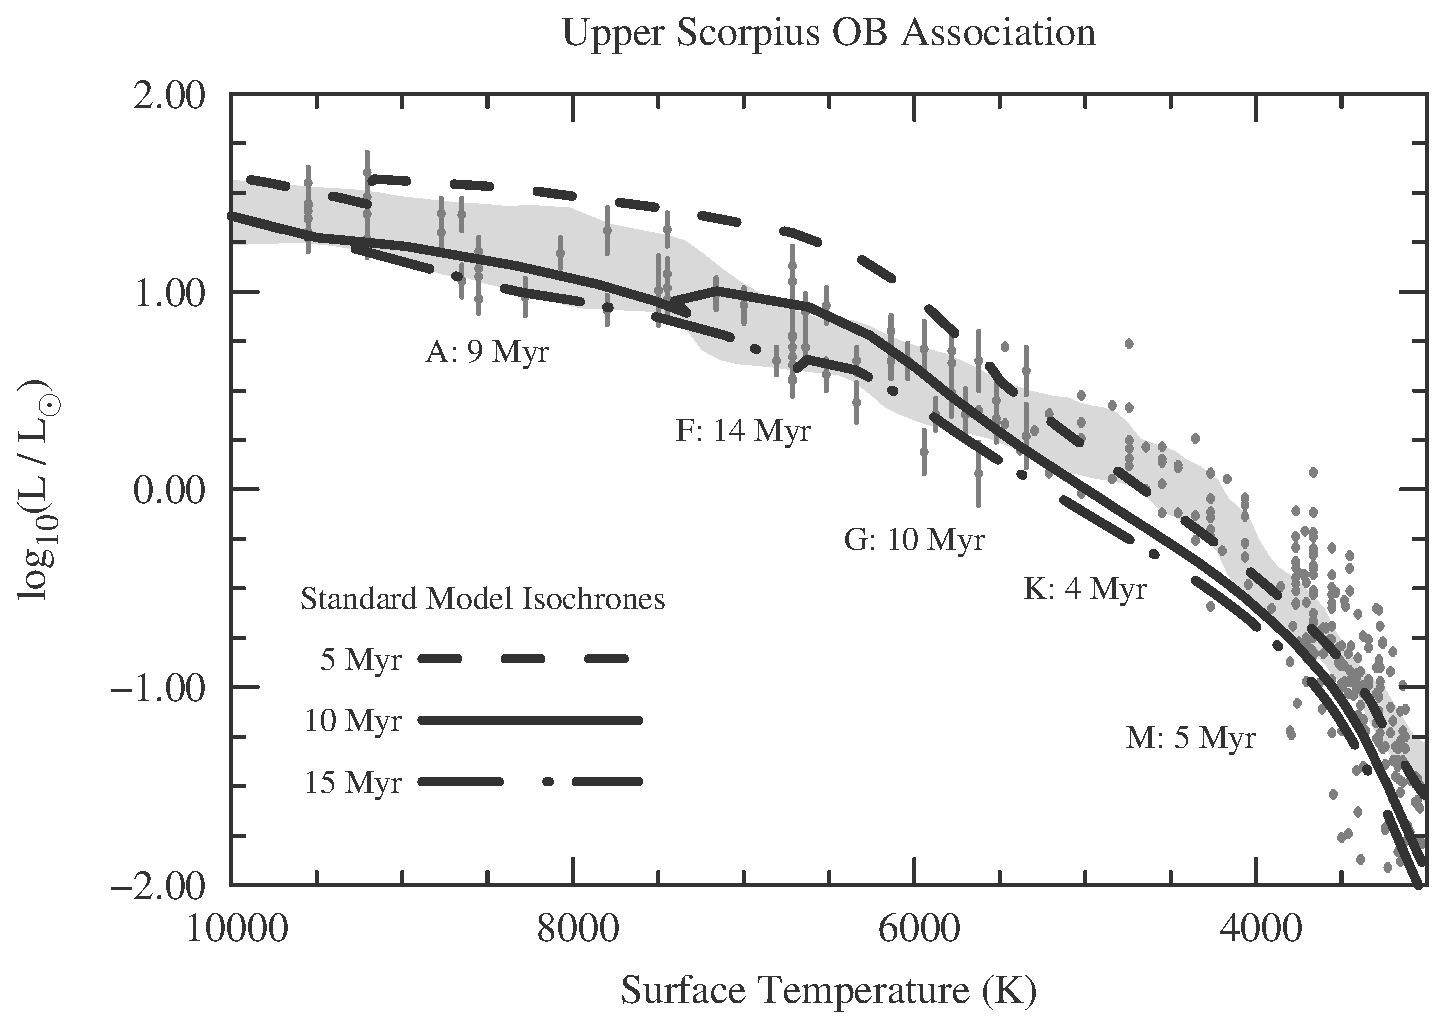
\includegraphics[width=0.65\columnwidth]{fig/USco_Age_Problems.eps}
	\caption{HR diagram for the Upper Scorpius OB Association. Stellar evolution model isochrones are shown in black. Labels show the ages inferred from different sub-populations in the association, highlighting a clear discordance between ages of hot and cool stars.}
	\label{fig:badhrd}
	\vspace{-0.2in}
\end{figure}

The difficulty is identifying which physics are missing from the models. Several mechanisms have been proposed to explain the luminosity spreads observed in HRDs of the youngest clusters. Examples include episodic accretion \citep{Baraffe2009, Baraffe2010} and starspots \citep{Somers2015b}, which can cause intrinsic variations in luminosity among a coeval population of stars. Until recently, there had not been a convincing demonstration of a physical mechanism to explain the observed effective-temperature-dependent ages or to explain the discrepancies between HRD and MRD age estimates. There had only been speculation that was focused on the usual suspects that are blamed for uncertainties in stellar models: convection, radiative opacities, or the absence of magnetic fields and starspots  \citep{Stassun2014, Soderblom2014, Herczeg2015}. 

% without supporting evidence





%{\bf\large 2. Previous Work: Magnetic Fields in Early Stellar Evolution} \addcontentsline{toc}{section}{Previous Work: Magnetic Fields in Early Stellar Evolution} 
%
%
%\citet{DAntona2000} presented the first hints the missing physics, well before the full severity of model deficiencies was understood. They showed that including a rudimentary prescription for the effects of magnetic fields on convection provided better...

\begin{figure}
	\centering
    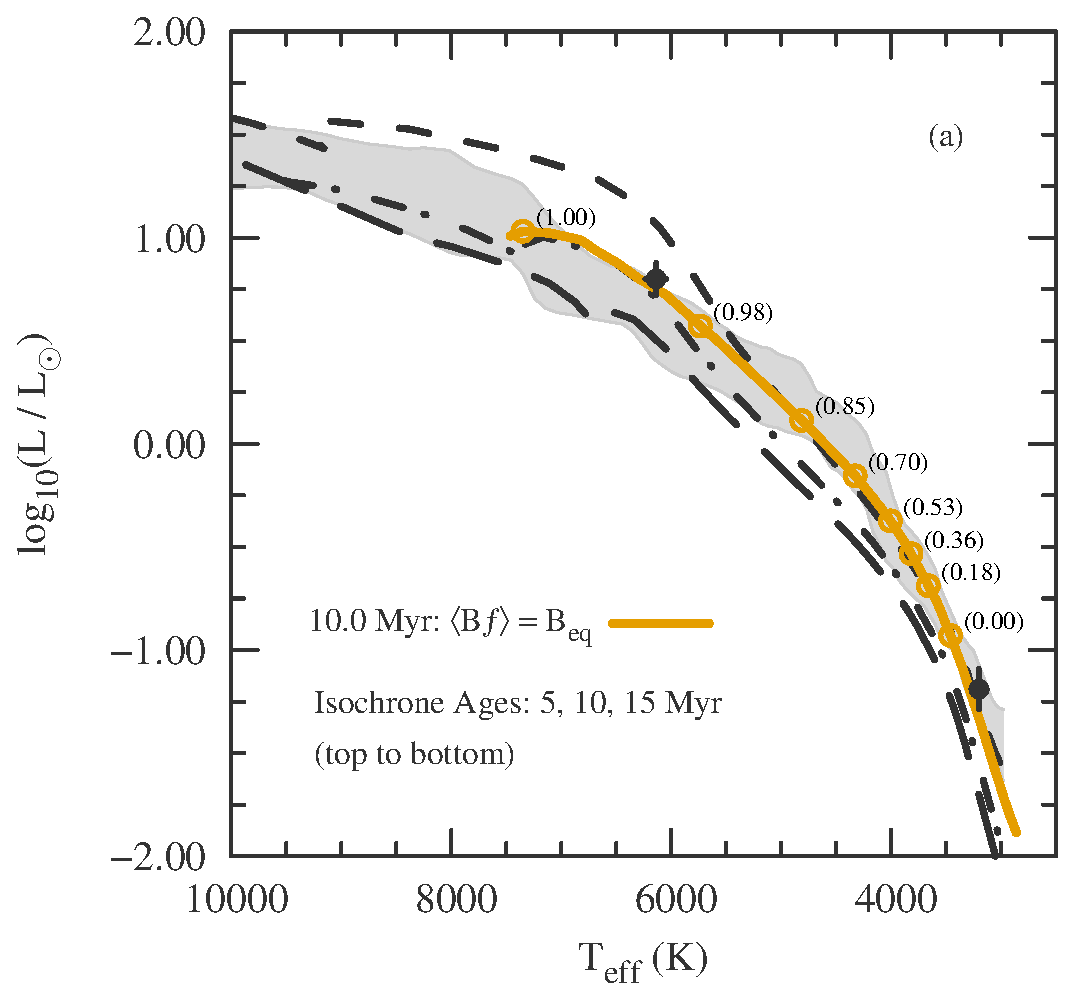
\includegraphics[scale=0.45]{fig/USco_HR_diagram.eps} \hspace{\fill}
    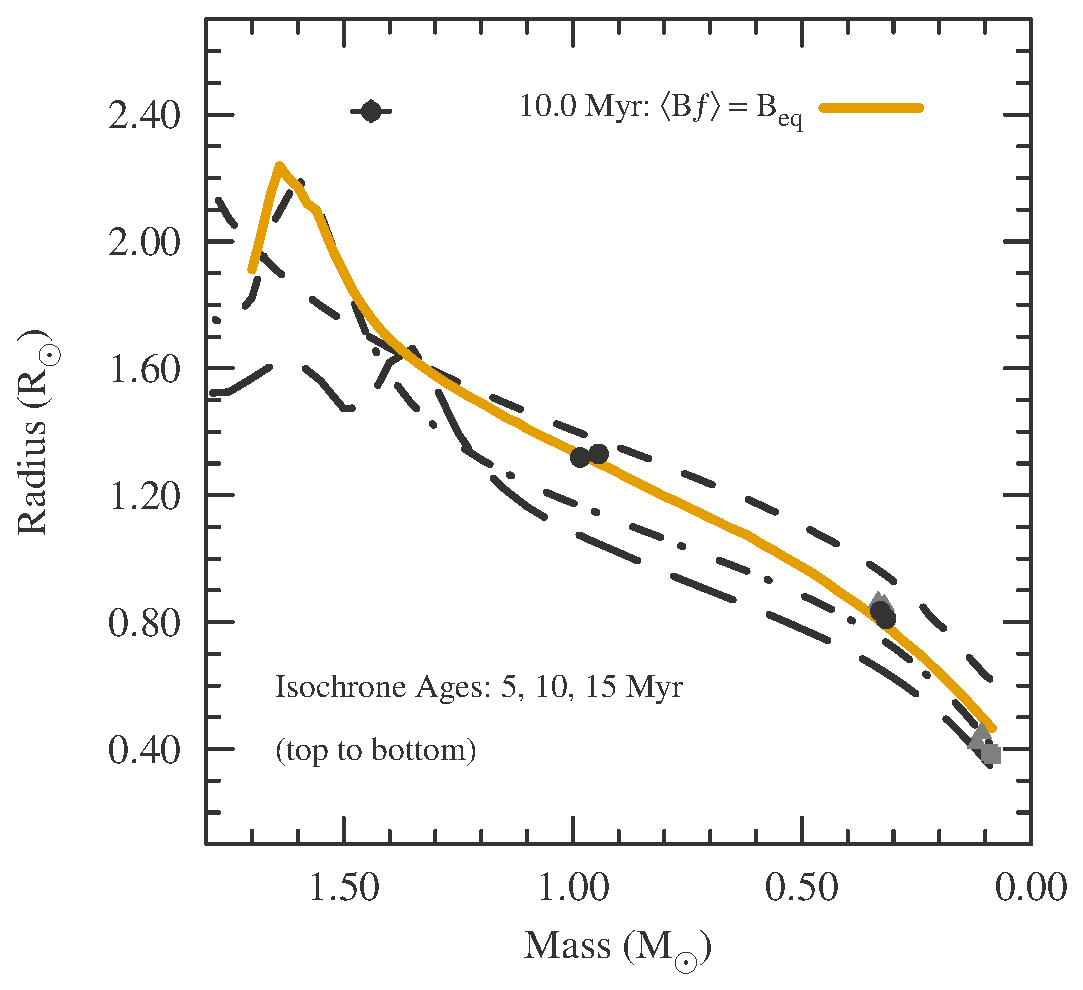
\includegraphics[scale=0.45]{fig/USco_MR_diagram.eps}
    \caption{({\it left}) HR diagram of Upper Scorpius with components of eclipsing binary systems UScoCTIO5 \citep{Kraus2015} and HD 144548 \citep{Alonso2015}
    observed by {\it Kepler}/K2 (black points). A 10 Myr magnetic stellar evolution isochrone is shown by the solid blue line. Note that the 10 Myr magnetic isochrone lies on top of the 5 Myr standard isochrone. ({\it right}) Mass-radius relationship for Upper Scorpius from {\it Kepler}/K2 eclipsing binary systems. {\it Unlike standard models, magnetic stellar evolution models naturally reproduce the slope of the low-mass mass-radius relationship at the same age predicted from the HR diagram.}}
    \label{fig:usco}
    \vspace{-0.2in}
\end{figure}

Recently, our group demonstrated that magnetic fields may provide a viable explanation for observed surface-temperature dependent ages in young clusters and the discordance between HRD and MRD age estimates \citep[see Figure~\ref{fig:usco};][]{Feiden2016}. The hypothesis is that Lorentz forces generated by strong magnetic fields suppresses convective flows in young stars, which acts to cool the stellar surface \citep[e.g.,][]{DAntona2000, MM01, FC12b}. As a result, the contraction of young pre-main-sequence stars is delayed, meaning young stars have cooler temperatures and larger radii at a given age when magnetic inhibition of convection is included in model calculations \citep{MM10, Feiden2016}. The physical mechanism is analogous to formation of sunspots, where strong magnetic fields suppress convection causing the stellar plasma contained within a magnetic region to cool and thus appear darker than its surroundings \citep{Biermann1941, Deinzer1965}. The difference is that sunspots are highly localized phenomena whereas our models consider global-scale magnetic inhibition of convection. 

Previous investigations showed that magnetic inhibition of convection could relieve age disparities between HRD ages and lithium depletion boundary ages \citep{DAntona2000}. For examples, ages inferred from an HRD for cool star members of the $\beta$ Pictoris moving group using standard stellar evolution models indicated the group was 10 Myr old \citep{Zuckerman2001}, while the same models provided an age of 20 Myr based on the lithium depletion boundary location \citep{Song2002, Binks2014}. However, by including magnetic inhibition of convection, \citet{MM10} and \citet{Malo2014} showed that the two age estimates could be brought into rough agreement at an age of 25 -- 30 Myr. Shortly thereafter, \citet{Mamajek2014} re-derived an age for high-mass members of the $\beta$ Pictoris moving group and found an age consistent with the magnetic model predictions for the ages of the cool stars. This provided the first hint that magnetism may explain effective-temperature-dependent ages.
%age discrepancies for the 25 Myr old $\beta$ Pictoris moving group \citep{MM10, Malo2014}.

Magnetic models were successful at reconciling the two age estimates, but it was not clear whether the magnetic models were {\it accurate} because HRD and lithium depletion boundary studies are mass agnostic. To know whether magnetic models predict accurate properties for real stars, EBs in well-studied young clusters were needed. Masses and radii directly measured for stars in EBs provide the most stringent test of stellar models as mass is the primary model input and observationally determined radii are more reliable than $T_{\rm eff}$ and luminosity estimates. Finding EBs in young clusters would also provide an opportunity to confirm the MRD age estimate against an age inferred from an HRD using an independent sample of stars.

A source of EBs in a well-studied young cluster became available when \kepler\ observed the Scorpius-Centaurus OB Association for 80 continuous days. A number of EBs were quickly identified in the Upper Scorpius subgroup, including two EBs for which precise masses and radii were determined \citep{Kraus2015, Alonso2015}. Critically, the two EBs occupied two distinct regions of the MRD thereby defining a preliminary mass-radius relationship (see Figure~\ref{fig:usco}). Comparing the EB mass-radius relation against model predictions, it is clear that standard models predict an incorrect {\it slope} for the mass-radius relationship. Ultimately, models were found to exhibit errors in age by up to 100\% and using the empirical HRD to derive a mass from standard models yields errors in the true mass by up to 50\% \citep{Kraus2015}.

However, when we compare the mass-radius relationship predicted by models that include magnetic inhibition of convection, we find that the model mass-radius relation steepens such that it closely matches the observed relationship at an age of approximately 10 Myr \citep[see Figure~\ref{fig:usco};][]{Feiden2016}. Figure~\ref{fig:usco} also demonstrates that the age predicted by the magnetic models in the MRD provides a reasonable fit to the median HRD sequence. {\bf Magnetic models appear to predict a consistent age in both the HRD and MRD. Furthermore, magnetic models predict an age that is largely independent of effective temperature in the HRD.} What's more, is that the surface magnetic fields strengths used to compute the stellar models were selected {\it a priori} based on arguments that the magnetic field is in thermal equipartition with the surrounding gas, as has been observed among young T-Tauri stars \citep{JohnsKrull1999}, and deep interior magnetic field strengths are of a plausible magnitude \citep{Browning2016}. This means magnetic models are exhibiting some level of predictive power when it comes to reproducing the properties of young stars.

% \citep{JohnsKrull1999}. 
%Results from \citet{Feiden2016} are tantalizing, as they offer a path toward reliable young stellar ages, but important questions remain about the validity and accuracy of these ``magnetic stellar evolution models.'' First, properties of the magnetic field are prescribed in a rather ad-hoc fashion \citep{FC12b, FC13}. Simple functions are used to describe the magnetic field strength as a function of radius deep in a star \citep{FC13}, but the situation in real stars is far more complex and depends intimately on the precise structure and rotational velocity of the star \citep{Browning2008, Brown2010}. Second, the interaction of Lorentz forces on convection depend strongly on the magnetic field topology throughout the star \citep{FC13}. At the moment, models use a free parameter to describe an average magnetic field topology, but the parameter is fixed and not allowed to vary as would be expected for a real magnetic field \citep{FC12b}. Finally, the existing magnetic field framework requires the specification of the surface magnetic field strength \citep{FC12b}. This value is either chosen arbitrarily \citep{FC12b, FC13, FC14, FC14b}, or at best, order of magnitude estimates are used to describe a possible maximum value \citep{Feiden2016}. The latter estimates are consistent with field strengths observed on young T Tauri stars \citep{JohnsKrull1999}, but this provide only indirect support for the model predictions.

%The full effect of these modeling choices are felt when stars are allowed to evolve in time. Properties of the magnetic field are a function of the stellar structure and stellar rotation, which both vary over time. Therefore, magnetic fields are expected to also evolve in time. 

Results from \citet{Feiden2016} are tantalizing, as they offer a path toward reliable young stellar ages, but important questions remain about the validity and accuracy of these ``magnetic stellar evolution models.'' Answers to some of these questions, such as whether model predict the correct mass-radius relationship across the entire MRD, are near at hand thanks to immense efforts to uncover and characterize EBs in young stellar populations with \kepler. However, detailed studies testing new hypotheses, such as magnetic inhibition of convection, are currently hampered by a lack of availability of models that incorporate these new physics (e.g., accretion, magnetic fields, starspots). To make real progress in understanding the observed discrepancies, theoretical models must be available to permit quantitative tests of predictions made by new models. \\


 
%a grid and tools to facilitate adoption of standard and magnetic models is needed to provide a means of testing and magnetic hypothesis.



\clearpage

{\bf\large 3. Proposed Research: Grids of Magnetic (sub)Stellar Evolution Models} \addcontentsline{toc}{section}{Proposed Research: Grids of Magnetic (sub)Stellar Evolution Models} \\


\bibliography{/Users/grefe950/Documents/papers}

\clearpage

%
%
% Name and header
{\bf\large 8. Biographical Sketches} \addcontentsline{toc}{section}{8. Biographical Sketches} \\

{\bf\large \noindent{Gregory A. Feiden}} \\
\hrule\vspace{\baselineskip}

% Education Section
\noindent{\bf Education}:
\begin{flushright}
    \begin{tabular*}{\linewidth}{l l @{\extracolsep{\fill}} r}
        2008 -- 2013  &  Ph.D. (Physics \& Astronomy)  &  Dartmouth College  \\
        2004 -- 2008  &  B.S. (Physics)  &  State University of New York at Oswego  
    \end{tabular*}
\end{flushright}
\vspace{0.4\baselineskip}

% Research Experience
\noindent{\bf Appointments}:
\begin{flushright}
	\begin{tabular*}{\linewidth}{l l @{\extracolsep{\fill}} r}
		2016 --        &  Assistant Professor of Astronomy & University of North Georgia \\
		2015 -- 2016   &  Research Scientist    &  Uppsala University \\
        2013 -- 2015   &  Postdoctoral Fellow   &  Uppsala University \\
        2012 -- 2013   &  Gordon F. Hull Graduate Fellow  &  Dartmouth College \\
		2011 -- 2012   &  Neukom Graduate Fellow & Dartmouth College \\
    \end{tabular*}
\end{flushright}
\vspace{0.4\baselineskip}

\noindent{\bf Awards}:
\begin{flushright}
	\begin{tabular*}{\linewidth}{l @{\extracolsep{\fill}} l r}
%	2014         & Uppsala University Rector's travel grant     & 19\,800 SEK \\
%    2014         & Swedish National Space Board travel grant  & 11\,000 SEK \\
    2013 -- 2015 & Uppsala U.\ Postdoctoral Fellowship, Physics \& Astronomy & 840\,000 SEK \\%
	2012 -- 2013 & Gordon F. Hull Graduate Fellowship  & 26\,000 USD \\    
    2011 -- 2012 & Neukom Institute for Computational Science Fellowship & 26\,000 USD
    \end{tabular*}
\end{flushright}
\vspace{0.4\baselineskip}

%\noindent{\bf Research Interests}: 
%\begin{flushright}
%    \parbox{0.99\linewidth}{
%	\noindent Physics of (sub)stellar interiors and atmospheres; Computational stellar evolution; Stellar ages; Convection; Magneto-convection; Stellar populations; Radiative transfer.}
%\end{flushright}
%\vspace{0.4\baselineskip}

\noindent{\bf Experience \& Expertise}:  %\hspace{\fill} {\small (see page 4)}
\begin{center}
	List everything here.
\end{center}
\vspace{0.4\baselineskip}

\noindent{\bf Relevant Publications}: % \hspace{\fill} {\small (see page 4)}
\begin{enumerate}
	\setlength{\itemsep}{0em}
	\item {\bf Feiden, G.~A.} {\it Magnetic Inhibition of Convection and the Fundamental Properties of Low-Mass Stars. III. A Consistent 10 Myr Age for the Upper Scorpius OB Association}, 2016, A\&A, in press.
	
	\item Mann, A.~W., Newton, E.~R., Rizzuto, A.~C., {Irwin}, J., 
	{\bf {Feiden}, G.~A.}, {Gaidos}, E., {Mace}, G.~N., {Kraus}, A.~L., 
	{James}, D.~J., {Ansdell}, M., {Charbonneau}, D., {Covey}, K.~R., 
	{Ireland}, M.~J., {Jaffe}, D.~T., {Johnson}, M.~C., 
	{Kidder}, B., \& {Vanderburg}, A. \emph{Zodiacal Exoplanets in Time (ZEIT) III: A Neptune-sized planet orbiting a pre-main-sequence star in the Upper Scorpius OB Association}, 2016, ApJ, in press. 
	
	\item Stassun, K.~G., {\bf Feiden, G.~A.}, \& Torres, G. {\it Empirical Tests of Pre--Main--Sequence Stellar Evolution Models with Young Eclipsing Binary Stars}, 2014, New Ast.\ Rev., 60, 1.
	
	\item Torres, G., Lacy, C.~H.~S., Pavlovski, K., {\bf Feiden, G.~A.}, {Sabby}, J.~A., {Bruntt}, H., \& {Viggo Clausen}, J. {\it The G+M Eclipsing Binary V530 Orionis: A Stringent Test of Magnetic Stellar Evolution Models for Low--Mass Stars}, 2014, ApJ, 797, 31.
	
	\item Malo, L., Doyon, R., {\bf Feiden, G.~A.}, {Albert}, L., 
	{Lafreni{\`e}re}, D., {Artigau}, {\'E}., {Gagn{\'e}}, J., \& 
	{Riedel}, A. {\it BANYAN. IV. Fundamental Parameters of Low-Mass Star Candidates in Nearby Young Stellar Kinematic Groups---Isochronal Age Determination Using Magnetic Evolutionary Models}, 2014, ApJ, 792, 37.
	
	\item  {\bf Feiden, G.~A.} \& Chaboyer, B. {\it Magnetic Inhibition of Convection and the Fundamental Properties of Low-Mass Stars. II. Fully Convective Main Sequence Stars}, 2014, ApJ, 787, 53.
	
	\item  {\bf Feiden, G.~A.} \& Chaboyer, B. {\it Magnetic Inhibition of Convection and the Fundamental Properties of Low-Mass Stars. I. Stars with a Radiative Core}, 2013, ApJ, 779, 183.
	
	\item {\bf Feiden, G.~A.} \& Dotter, A. {\it The Interior Structure Constants as an Age Diagnostic for Low-Mass, Pre-Main-Sequence Detached Eclipsing Binary Stars}, 2013, ApJ, 765, 86.
	
	\item {\bf Feiden, G.~A.} \& Chaboyer, B. {\it Self-Consistent Magnetic Stellar Evolution Models of the Detached, Solar-Type Eclipsing Binary EF Aquarii}, 2012, ApJ, 761, 30.
	
	\item \textbf{Feiden, G.~A.} \& Chaboyer, B. \emph{Reevaluating the Mass-Radius Relation for Low-Mass, Main Sequence Stars}, 2012, ApJ, 757, 42. 

\end{enumerate}
\vspace{\baselineskip}

\noindent{\bf Advisors and Advisees}:
\begin{flushright}
    \parbox{0.99\linewidth}{
	\noindent {\bf Graduate and Postgraduate Advisors:} Brian Chaboyer (Dartmouth), Nikolai Piskunov (Uppsala), Susanne H\"{o}fner (Uppsala) \\
	\noindent {\bf Graduate Advisees:} Steven Christophe (Paris-Sud / Uppsala) \\
	\noindent {\bf Undergraduate Advisees:} Jaquille Jones (Dartmouth), Jonas Engman (Uppsala) 
	}
	
\end{flushright}


\clearpage

%
%

{\bf\large 8. Current and Pending Support} \addcontentsline{toc}{section}{Current and Pending Support} 

{\bf 8.1 Gregory A.~Feiden} 

{\it 8.1.1 Current}

None 

{\it 8.1.2 Pending}

Title: ``The Exoplanet Migration Timescale from Young Clusters in K2'' \\
Admin PI: Dr. Adam L.\ Kraus \\
Science PI: Dr. Aaron C.\ Rizzuto \\
Program Name: ROSES-2016/Astrophysics Data Analysis Program \\
Sponsoring Agency: NASA \\
Contact: Douglas M. Hudgins, (202) 358-0988, Douglas.M.Hudgins@nasa.gov \\
Performance Period: 01/01/2017 -- 12/31/2018 \\
Total Budget: \$252,385.00 \\
Commitment by PI: < 1 month during the 2017 and 2018 academic years for determining stellar parameters using standard and magnetic models. Supported by the PI's 9 month salary. \\

Title: ``The Mass-Radius Relation of Young Stars from K2'' \\
Admin PI: Dr. Adam L.\ Kraus \\
Science PI: Dr. Adam L.\ Kraus \\
Program Name: ROSES-2016/Astrophysics Data Analysis Program \\
Sponsoring Agency: NASA \\
Contact: Douglas M. Hudgins, (202) 358-0988, Douglas.M.Hudgins@nasa.gov \\
Performance Period: 01/01/2017 -- 12/31/2018 \\
Total Budget: \$234,545.00 \\
Commitment by PI: < 1 month during the 2018 academic year to provide custom models with magnetic fields. Supported by the PI's 9 month salary. \\

\end{document}